\section{Soll-Zustand}
Der Ist-Zustand beschrieben in Kapitel \ref{sec:Istzustand} hat gezeigt, dass viele manuelle Tätigkeiten für die Beladung und Abfertigung, sowie die Rangiervorgänge von Güterwagen im Einzelwagenverkehr notwendig sind.\par
Dies verursacht hohe Kosten durch die benötigte Zeit (siehe dazu auch den Zeitvergleich in Abbildung \ref{fig:Zeitvergleich} auf Seite \pageref{fig:Zeitvergleich}) und das benötigte Personal, sowie auch Kosten an der Verladestelle, wenn diese aufgrund von Kupplungs- und Rangiervorgängen belegt ist.\par
Zur besseren Einordnung sollen nun diese Komponenten definiert und erläutert werden aus denen sich verschiedene Stufen ergeben und aus denen sich wiederum später verschiedene Anforderungen ergeben.\par
Eine Aufteilung findet in Anlehnung an den Projektantrag statt. \textbf{Nach kurzen Vorbemerkungen wird zu Beginn das Gesamtsystem vorgestellt. Danach findet eine Aufteilung nach ABC statt.}
\subsection{Vorbemerkungen}
Bei einem Umbau für die Demonstratoren muss darauf geachtet werden, dass ein voll- ständiger Rückbau der neuen Einrichtungen möglich ist, aber auch so bahntauglich ist, dass die Demonstratoren für ein Folgeprojekt oder Feldversuche genutzt werden können. Diese Projekt muss nicht sofort zulassungsfähig sein, sollte aber eine Basis dazu bilden. \par
An der Bewegung der Wagen im Wagenverband an sich mit Hilfe einer Lok oder eines anderen Rangierhilfsmittel soll hier nichts automatisiert werden. Siehe dazu auch in den Kapiteln \ref{sec:Zustellfahrt}, \ref{sec:Zugfahrt} und \ref{sec:Rangierfahrt}. Automatisierungen können und sollen aber selbst verständlich im Bereich der Kupplung, Bremse oder auch der informationstechnischen Prozesse stattfinden.\par
Wie in Kapitel \ref{sec:Personal} angedeutet und in Kapitel \ref{sec:LuftumechKup} beschrieben, ist das mechanische Kuppeln und das Kuppeln von Luft aufwendig, körperlich anstrengend und fehlerbehaftet. \par
Zur Automatisierung von mechanischen Kupplungen gibt es Kupplungsrobotoren\footnote{Zum Beispiel die Bahn-Kupplungs-Robotoren BaKuRo und EntKuRo}. Alternativ ist die Automatische Kupplung \acrshort{AK} eine Lösung, aber auch nach deren Einführung im vorigen Jahrhundert ist eine flächendeckende Nutzung im Güterverkehr noch nicht realisiert.\par
Aufgrund dieser Punkte ist es erst einmal sinnvoll mit der mechanischen Kupplung weiter zu machen und Lösungen für die \acrshort{AK} kompatibel zu halten. Eine starke Vereinfachung würden die bereits in den vorigen Abschnitten beschriebene automatische Bremse mit ihren fernstellbaren Ventilen bringen.

\subsection{Gesamtsystem}
Das Gesamtsystem besteht aus den Komponenten des Güterwagens. Der Güterwagen 4.0 soll im Vergleich zum konventionellen Güterwagen eine aktive Rolle in der Zugvorbereitung und an der Ladestelle spielen. Dafür ist eine Stromversorgung, Telematik und Datenvernetzung zu anderen Güterwagen sowie Logistiksystemen notwendig. Zusätzlich soll ein Automatisierung der Bremsbedienung stattfinden. Ist hier eine sichere Übertragung über den gesamten Zug, auch bei der Fahrt, möglich, ist auch eine ep-Bremse möglich. Diese Punkte sollen auch in diesem Projekt bereits umgesetzt werden. Weitere Punkte, die in Folgeprojekten umgesetzt werden sollen, ist ein automatisierter Zugschluss und ein Rangierantrieb.\par
In Kapitel \ref{sec:BewdWagen} werden die verschiedenen Möglichkeiten der Wagenbewegung betrachtet. Im Allgemeinen werden dafür zusätzliche Fahrzeuge, Personal und eine Gleisanlage benötigt. Je nach Beschaffung der Gleisanlage und die in Kapitel \ref{sec:Fahrweg} angesprochene Einschränkung, werden zusätzliche Sägefahrten zur korrekten Einsortierung der Wagen auf verschiedene Gleise benötigt. \par
Ein eigener Antrieb auf jedem Wagen, der eine selbstständige Bewegung in geringer Geschwindigkeit zulässt wäre hier eine Lösung.\par
Einfach ist diese Lösung allerdings nicht. Hier müssen vor allem die Punkte des eigenen Antriebs, der darauf ausgelegten Stromversorgung und der dazu passenden Aufladung der Batterien und die Sicherheitsansprüche beachtet werden. Darum ist eine Umsetzung in diesem Projekt noch nicht gaplant.\par
Das Abdrücken am \gls{Ablaufberg}, siehe Kapitel \ref{sec:Abdruecken} ist bereits auf großen Rangierbahnhöfen automatisiert, siehe Kapitel \ref{sec:automAbdruecken}. Dennoch ist auch hier Handarbeit zur Vorbereitung notwendig. Die Wagen müssen vorentkuppelt werden, das bedeutet hier, dass die Luftlupplung gelöst wird und die mechanische Kupplung nur noch eingehakt wird. Der Wagen wird dann wieder mittels Hemmschuh festgelegt und kurz vorm \gls{Ablaufberg}, vom Stangler, vollständig entkuppelt. Hier soll mittels Zustandsanzeige der Bremse die Vorentkupplung vereinfacht werden. Dank automatischer Feststellbremse werden dann auch keine Hemmschuhe mehr benötigt.

\subsubsection{Stromversorgung, Telematik und Datenvernetzung}
Alle elektrischen Komponenten arbeiten mit 24 V. 

\subsubsection{Automatisierte Bremsbedienung}
Die Einführung einer automatischen Bremse soll vor allem zur Zeitersparnis bei der Zugvorbereitung und \gls{Bremsprobe} führen.\par
Besonders wichtig zur Einführung der automatisierten Bremse ist die Fernbetätigung dieser. Sie sollte vor allem die Möglichkeiten zum Schnelllösen, Aus- und Einschalten der Bremse, Änderung der Bremsstellung und Einstellen der Feststellbremse (auch automatische Parkbremse) haben.
Durch ein TSI-konformes Steuerventil soll die Umstellung der Bremsarten mittels G/P-Umsteller automatisiert werden. Auch eine automatische Lastabbremsung mittels Wiegeventil ist vorgesehen. Hier ist bei beiden Funktionen vor allem auf eine sichere Funktion und Rückmeldung zu achten.
Für diese sichere Übertragung ist die Messung des C-Drucks von größter Wichtigkeit.
Auch fernbetätigte Absperrhähne sollen zu dieser Zeiteinsparung führen. 
Da der Zustand der Bremse nicht mehr zwangsläufig von außen sichtbar ist, ist eine Bremszustandsanzeige am Wagen anzubringen. 

\subsubsection{ep-Bremse}
Durch eine Automatisierung der Bremse ist nun auch eine ep-Bremsung möglich.

\subsubsection{sonstige Punkte}

\subsection{Sensorik}
\textbf{Hier muss was hin}
\subsubsection{Messung C-Druck}
Der Bremszylinderdruck (C-Druck) wird gemessen. 
%2.	Der Sensor arbeitet als Stromsensor (4-20 mA).
%3.	Der Messbereich ist (0...5) bar.
Die Messunsicherheit und Auflösing ist so gewählt, dass die erste und letzte Bremsstufe %(0,45 bar Cv) 
sicher erkannt werden. %Eine Messunsicherheit von 0,05 bar erfüllt diese Anforderung.

\subsection{Aktorik}
\textbf{Hier muss was hin}
\subsubsection{Fernbetätigung Bremse}
Die Fernbetätigung der Bremse soll vor allem die Zeit des Entlanglaufens des Zuges beim Prüfen der Bremse ersparen. Es müssen folgende Funktionen fernbetätigt werden können:
\begin{itemize}
    \item Schnelllösen
    \begin{itemize}
        \item Ein Löseimpuls löst die Schnelllösefunktion des Steuerventils aus.
        \item Der Löseimpuls kann elektromechanisch oder pneumatisch auf das Steuerventil übertragen werden.
    \end{itemize}
    \item Bremse aus
    \begin{itemize}
        \item Die Funktion ist bistabil umzusetzen.
        \item 	Es werden folgende Verbindungen geöffnet bzw. geschlossen:
        \begin{itemize}
            \item HLL - SV (Entlüftung zum SV)
            \item SV - R (Entlüftung zum SV)
            \item SV - Cv (Entlüftung zum Relaisventil)
        \end{itemize}
        \item Die Betätigung muss in weniger als 10 Sekunden durchgeführt werden.
    \end{itemize}
    \item Bremsstellung
    \begin{itemize}
        \item Die Bremsstellung wird elektrisch bistabil durch Verstellen des SV umgestellt.
        \item Eine Rückmeldung ist vorzusehen.
    \end{itemize}
    \item Festellbremse
    \begin{itemize}
        \item Die Feststellbremse kann unabhängig von der pneumatischen Energie im Wagen angelegt und gelöst werden.
        \item Das Anlegen und Lösen erfolgt bistabil durch eletrischen Impuls.
        \item Eine Rückmeldefunktion für den gelösten Zustand ist vorzusehen.
        \item Die Bremskraft am Bremszylinder beträgt ??kN (für 2\%-Gefälle, 90 t, Klotzbremse).
        \item Alternative Lösungen, wie Federspeicher oder FT Park Lock können vorgeschlagen werden
        \item mit Luft = ungebremst, ohne Luft = gebremst
    \end{itemize}
\end{itemize}
\subsubsection{Steuerventil}
Die Bremsarten G und P sollen mittels Aktor sicher umgestellt und detektiert werden. Auch eine Übertragung der aktuellen Stellung soll sicher gemeldet werden. Aus Zulassungsgründen soll ein UIC/TSI-kompatibels Steuerventil eingesetzt werden. Dieses verfügt dann über die Bremsstellungen G und P, über automatisches Schnelllösen. \par
Ein zusätzliches Relaisventil ist für die automatische Lastabbremsung mittels Wiegeventil vorgesehen. Dieses ist vorzugsweise nicht im Steuerventil integriert.
\subsubsection{Fernbetätigte Absperrhähne}
Die Endabsperrhähne sind bistabil, d.h. verbleiben ohne Betätigung in ihrem letzten Zustand. Ein freier Querschnitt von 1,25'' wird für sinnhaft erachtet. Die Betätigungszeit für den Übergang Öffnen-Schließen beträgt maximal 60 s. Die Hähne sind von ihrem Funktionsprinzip für Anforderungen nach DIN EN 14601 geeignet, diese muss allerdings noch nicht von Demonstratoren und Labormuster erfüllt sein. Eine fahrzeugseitige Verschraubung nach G1 1$/$4i (DIN EN ISO 228-1) ist zu bevorzugen. Für den Demonstrator kann die Kompatibilität durch einen Adapter hergestellt werden. Kupplungsseitig ist eine Verschraubung mit Whitworth-Gewinde mit stumpfen Gewinden für G1 1$⁄$4i—Leitungen zu bevorzugen. Für den Demonstrator kann die Kompatibilität durch einen Adapter hergestellt werden.
Gleichzeitig sollte der Wagen erkennen ob er in einem Wagenverbund oder alleine ist. Sollte er in einem Wagenverbund unterwegs sein, ist der Normalzustand für einen Wagen, dass die HL-Absperrventile die mit einem weiteren Wagen verbunden sind, offen sind und HL-Absperrventile am Rand des Zuges geschlossen sind.
\subsubsection{ep-Bremse}
Das ep-Brems-Ventil wird mit der HLL verbunden und zum Bremsen bestromt. Das Ventil entlüftet die HLL im Wagen in (3,5...5) s von Regelbetriebsdruck auf 3,5 bar.\par
Vorteile von ep-Bremsen sind, dass längere Züge möglich sind, weil die Zeit die die hinteren Wagen brauchen um die Absenkung des Luftdrucks mitzubekommen verkürzt wird. So drücken die sich noch schneller bewegenden Wagen weniger auf die sich langsamer bewegenden Wagen. Dies reduziert Verschleiß und sit nachhaltiger weil weniger Beschleunigungszyklen notwendig sind. Auch wird die Wartung, der Abrieb und die Gefahr von Flachstellen verringert.\par
Solange die ep-Bremse nicht auf die Bremshundertstel angerechnet wird, bedeutet sie auch keine Veränderung der Sicherheit. Soll sie angerechnet werden ist ein Nachweis über mindestens die gleiche Sicherheit notwendig.

\subsection{Kommunikation}
\textbf{Hier muss was hin}
\subsubsection{Zustandsanzeige Bremse}
\begin{figure}[htbp]
    \centering
    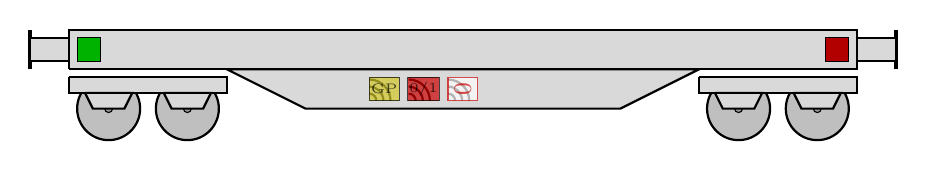
\begin{tikzpicture}[font = \sffamily]
%        \node (a) at (0,0) {};
%        \node (b) at (6,0) {};
        \draw[fill = gray!30, thick] (0,3) -- (10,3) -- (10,3.5) -- (0,3.5) -- (0,3);
        \draw[fill = gray!30, thick] (2,3) -- (3,2.5) -- (7,2.5) -- (8,3) -- (2,3);
        %DG 1
        \draw[fill = gray!50, thick] (8.5, 2.5) circle[radius = .4cm];
        \draw[fill = gray!80] (8.5, 2.5) circle[radius = .05cm];
        \draw[fill = gray!50, thick] (9.5, 2.5) circle[radius = .4cm];
        \draw[fill = gray!80] (9.5, 2.5) circle[radius = .05cm];
			\draw[fill = gray!30, thick] (8,2.9) -- (10,2.9) -- (10,2.7) -- (8,2.7) -- (8,2.9);
			\draw[fill = gray!30, thick] (8.2,2.7) -- (8.3,2.5) -- (8.7,2.5) -- (8.8,2.7) -- (8.2,2.7);
			\draw[fill = gray!30, thick] (9.2,2.7) -- (9.3,2.5) -- (9.7,2.5) -- (9.8,2.7) -- (9.2,2.7);
        %DG 2
        \draw[fill = gray!50, thick] (0.5, 2.5) circle[radius = .4cm];
        \draw[fill = gray!80] (0.5, 2.5) circle[radius = .05cm];
        \draw[fill = gray!50, thick] (1.5, 2.5) circle[radius = .4cm];
        \draw[fill = gray!80] (1.5, 2.5) circle[radius = .05cm];
			\draw[fill = gray!30, thick] (0,2.9) -- (2,2.9) -- (2,2.7) -- (0,2.7) -- (0,2.9);
			\draw[fill = gray!30, thick] (0.2,2.7) -- (0.3,2.5) -- (0.7,2.5) -- (0.8,2.7) -- (0.2,2.7);
			\draw[fill = gray!30, thick] (1.2,2.7) -- (1.3,2.5) -- (1.7,2.5) -- (1.8,2.7) -- (1.2,2.7);
	%Puffer 2
			\draw[ultra thick] (10.5,3) -- (10.5, 3.5);
			\draw[fill = gray!30, thick] (10.5,3.1) -- (10,3.1) -- (10,3.4) -- (10.5,3.4) -- (10.5,3.1);
	%Puffer 2
			\draw[ultra thick] (-.5,3) -- (-.5, 3.5);
	 		\draw[fill = gray!30, thick] (-.5,3.1) -- (0,3.1) -- (0,3.4) -- (-.5,3.4) -- (-.5,3.1);
			% Neues UIC-Zeichen
			%\node [cloud, cloud puffs=9, draw = none, fill = yellow!80!black, minimum width=.8cm, minimum height=.3cm, font = \tiny, inner sep = 0] at (4, 3.25) {4.0};
			% Aussenanzeigen
			\draw[fill = green!70!black] (0.1,3.1) -- (0.4,3.1) -- (0.4,3.4) -- (0.1,3.4) -- (0.1,3.1);
			\draw[fill = red!70!black] (9.9,3.1) -- (9.6,3.1) -- (9.6,3.4) -- (9.9,3.4) -- (9.9,3.1);
			%\node[draw, fill = white, font = \small, inner sep = 0.6, minimum height = 0.3cm] at (4, 3.25) {P 86};
			\draw[thick] (3.90, 2.6) arc (0:90:.09cm);
			\draw[thick] (3.99, 2.6) arc (0:90:.18cm);
			\draw[thick] (4.08, 2.6) arc (0:90:.27cm);
			\node[opacity = .7, draw, fill = yellow!80!black, font = \tiny, inner sep = 0.6, minimum height = 0.3cm, minimum width = 0.38cm] at (4, 2.75) {GP};
			\draw[thick] (4.40, 2.6) arc (0:90:.09cm);
			\draw[thick] (4.49, 2.6) arc (0:90:.18cm);
			\draw[thick] (4.58, 2.6) arc (0:90:.27cm);
			\node[opacity = 0.7, draw, fill = red!80!black, font = \tiny, inner sep = 0.6, minimum height = 0.3cm, minimum width = 0.38cm] at (4.5, 2.75) {0/1};
			\draw[thick] (4.90, 2.6) arc (0:90:.09cm);
			\draw[thick] (4.99, 2.6) arc (0:90:.18cm);
			\draw[thick] (5.08, 2.6) arc (0:90:.27cm);
			\node[opacity = 0.7, draw = red!80!black, text = red!80!black, fill = white, font = \small, inner sep = 0.6, minimum height = 0.38cm, minimum width = 0.3cm, rotate = 90] at (5, 2.75) {0};

\end{tikzpicture}

    \caption{Zustandsanzeige Bremse \cite{ETR_3}}
    \label{fig:ZustandBremse}
\end{figure} 
Da der Zustand der Bremse nicht mehr zwangsläufig von außen sichtbar ist, siehe dazu Abbildung \ref{fig:ZustandBremse}, ist eine Bremszustandsanzeige am Wagen anzubringen. Hier ist mindestens eine Anzeige je Fahrzeugende zum Einbau am Pufferträger ist vorzusehen, so dass
 der Zustand der Bremse im Drehgestell immer zu erkennen ist. Die Anzeige stellt den Zustand der Bremskupplung (drucklos/druckbeaufschlagt) dar. Die Anzeige muss Überdrücke %> 0,5 bar 
 in den Bremskupplungen anzeigen, bspw. durch die Farbe "Rot'' im Schauglas. Bei Unterschreiten des Drucks wird bspw. die Farbe "Grün'' angezeigt. Die Anzeige muss auch im stromlosen Zustand verfügbar sein.
\subsubsection{Bremshundertstel/Bremsberechnung}
Die Bremshundertstel werden bisher, genau wie das Bremsgewicht, händisch mittels Bremszettel berechnet. Auf diesem Vordruck trägt der Triebfahrzeugführer Achszahl, Zugmasse und Bremsgewichte des Zuges ein. Daraus berechnen sich die Bremshundertstel. Nach Vergleich dieser mit den Mindest-Bremshundertstel der Strecke, ergibt sich Höchstgeschwindigkeit und Bremsstellung. die Bremsstellung wird nach jeder neuen Zusammenstellung und vor Fahrtantritt, siehe Kapitel \ref{sec:UEdWagen}, neu berechnet.\par
Diese manuelle Berechnung ist für Triebfahrzeugführer tägliche Arbeit, dennnoch ist sie Fehleranfällig und kann durch Rechnereinsatz einfach automatisiert werden.
\subsubsection{Bremsprobe}
\textbf{SIL-Bewertung - liegt nicht an, liegt an, sicheres lösen, sicheres stellen}.\par
Die \gls{Bremsprobe} findet zur Vorbereitung einer Sperr-, Rangier- oder Zugfahrt statt und überprüft die Funktionsfähigkeit des Bremssystems im Zug- oder Wagenverbund.\par
Sie wird von \gls{Bremsprobeberechtigte}n nach genau vorgeschriebenem Ablauf durchgeführt. Ja nach Zustand des Zuges und Fälligkeit der \gls{Bremsprobe} wird eine volle, vereinfachte, stationäre oder Führerraumbremsprobe durchgeführt. Der genaue Ablauf ist in der \acrshort{RIL} 915 oder der VDV-Schrift 757 geregelt.\par
\begin{figure}[htbp] 
    	\begin{center}
            		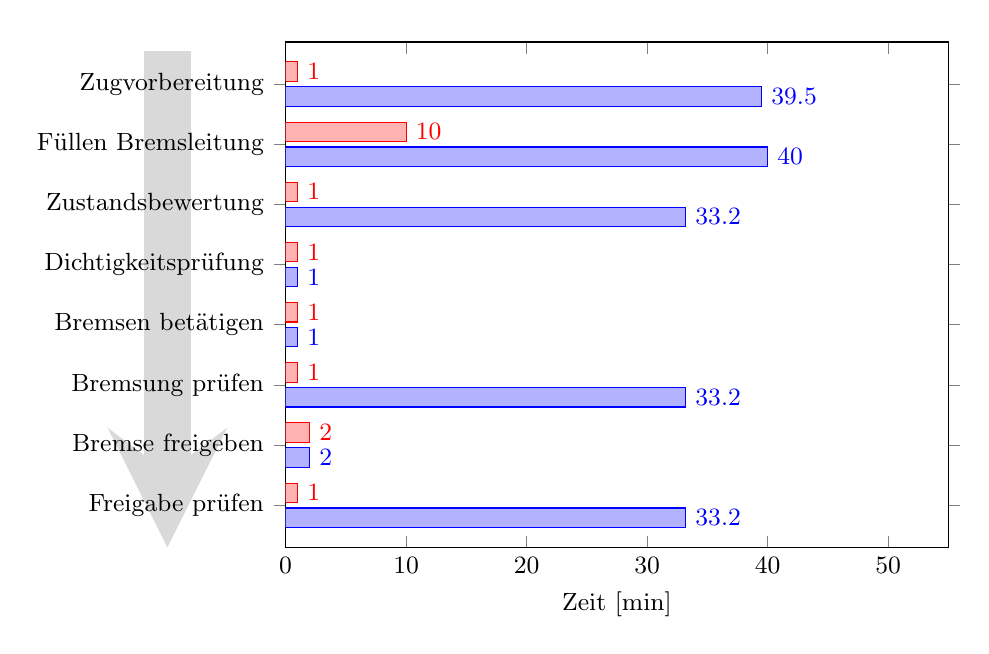
\begin{tikzpicture}[scale = 1]
		\draw[line width = .6cm, gray!30, -stealth] (-1.5,6.3) -- (-1.5,0);
                                \begin{axis}[ 
                                font = \small,
                                width = 10cm, height = 8cm,
                                xbar, xmin=0, xmax = 55,
                                xlabel={Zeit [min]},
                                symbolic y coords={%
                                {Freigabe prüfen},{Bremse freigeben},{Bremsung prüfen}, {Bremsen betätigen}, {Dichtigkeitsprüfung}, {Zustandsbewertung},{Füllen Bremsleitung},{Zugvorbereitung} },
                                ytick=data,
                                nodes near coords, 
                                %nodes near coords align={horizontal},
                                ytick=data,
                                % nodes near coords align={vertical},
                                bar width=7pt,
                %            legend style={
                   %             at={(1,1.1)},
                    %      	anchor=east},
                  %              legend columns = 2,
                                ]
                                \addplot coordinates {                          
                                (39.5,{Zugvorbereitung})
                                (40,{Füllen Bremsleitung})
                                (33.2,{Zustandsbewertung})
                                (1,{Dichtigkeitsprüfung})
                                (1,{Bremsen betätigen})
                                (33.2,{Bremsung prüfen})
                                (2,{Bremse freigeben})
                                (33.2,{Freigabe prüfen})
%                                (183.1,{Sum})
                                };
                                %\addlegendentry{Wagon $<$ 4.0}
                                \addplot coordinates {                          
                                (1,{Zugvorbereitung})
                                (10,{Füllen Bremsleitung})
                                (1,{Zustandsbewertung})
                                (1,{Dichtigkeitsprüfung})
                                (1,{Bremsen betätigen})
                                (1,{Bremsung prüfen})
                                (2,{Bremse freigeben})
                                (1,{Freigabe prüfen})
%                                (18,Sum)
                                };
                                %\addlegendentry{Wagon 4.0}
                                \end{axis}
                              \end{tikzpicture}
        		\end{center}
    \caption{Zeitvergleich Bremsprobe und automatisierte Bremsprobe nach \cite{Stephenson}}
    \label{fig:Zeitvergleich}
\end{figure} 
Abbildung \ref{fig:Zeitvergleich} zeigt einen Zeitvergleich zwischen konventioneller \gls{Bremsprobe} (blau) und automatisierter \gls{Bremsprobe (rot)}. Hier sieht man vor allem, dass  bei Zugvorbereitung, Füllen der Bremsleitung, Zustandsbewertung der Wagen und Überprüfung ob die Bremsen angelegt und wieder gelöst haben viel Zeit eingespart werden kann.
\textit{Durch bekannte Vorprüfungen kann die vollständige \gls{Bremsprobe} vereinfacht werden. Zum Beispiel durch sogenannte vorgeprüfte Gruppen.\\
\textbf{Siehe auch DI, Luftventile\\
\ref{sec:vBremsprobe}, \ref{sec:UEdWagen}, \ref{sec:RangKnoten}}}
\textbf{Siehe auch Bremsprobe im Anhang}
\subsubsection{Transportdokumente}
Wie bereits In Kapitel \ref{sec:Transdoc} beschrieben, gibt es die papierlose Transportabwicklung inklusive Gefahrgutdokumenten bisher im LKW-Bereich, allerdings nicht im Bahnsektor. Ein Grund dafür ist die fehlende Dateninfrastruktur.\par
Durch eine durchgängige Stromversorgung auf dem Wagen und einen bahntauglichen Rechner sowie entsprechende Datenverbindungen kann dieses Problem angegangen werden.\par
\textit{\textbf{Siehe dazu auch:} Stromversorgung, Rechner, Datenverbindung, DI (Digitale Identität)}
\subsubsection{Zugvorbereitung}
\subsubsection{Digitale Identität}
\subsubsection{Rechner}
\subsubsection{Datenverbindung}

\subsection{Power-Management}
Wie lange muss die Batterie durchhalten? Welche Verbraucher hängen daran?


\subsection{Sicherheitsanforderungen}
Die Sicherheit muss mindestens genauso bleiben, wie sie beim bisherigen System ist.\par
Eine sichere Übertragung der Zugintegrität ist in diesem Projekt nicht geplant.

\subsection{Migration}
ine große betriebliche Herausforderung besteht in der Tatsache, dass GW40 planmäßig oder unplanmäßig in ZBA auftauchen können. Sollten Sie dort den Betrieb stören, wäre das das Aus für ein solches Konzept.\par
Worst-case Szenario. Es gibt kein Strom. Nur Hilfsbedienungen möglich. Diese müssen an geeigneter Stelle (Chassis-Unterseite) durch einen Schlüssel durchgeführt werden. Dieser Schlüssel muss nicht individuell sein. Er kann in der Anlage standardmäßig vorhanden sein oder (wie der Nothammer im ÖPNV) in einem verplombten Halter sein.\par
Man kann mit diesem Schlüssel alle Bedienhandlungen (Bremse ein/aus, Zugschluss, G/P, Last) vornehmen. Die Handbremse allerdings nicht. Der Wagen hat in diesem Szeanrio keinen Handbremse.\par
Um dieses Szenario immer verfügbar zu haben, findet sich an geeigneter Stelle eine Anweisung für den Notfall in den UIC-Sprachen und mit Pictogrammen. \par
Sobald der Wagen wieder Energie hat, also nach den ersten paar Metern Rangier- oder Zugfahrt, wird folgendes geprüft und eine entsprechende Statusmeldung in die Cloud gesandt.
\begin{itemize}
\item Notschlüssel entnommen / wieder vorhanden
\item Übereinstimmung der Ventilstellungen mit dem Steuerungsstatus
\end{itemize}
In Abhängigkeit der Überprüfung kann der nächsten Behandlungsstelle eine Warnung oder Information gegeben werden, was mit dem Wagen geschehen sollte.\par
Normales Szenario in der Migrationsphase. Außer einer generellen Bedienungsanweisung ist in der Behandlungsstelle nichts über die Eigenschaften des Wagens bekannt. Geringfügiger Nutzen ist vorhanden. Jede normale Bedienhandlung ist durch Tastenbedienung mit Leuchtmelderrückmeldung ersetzt.\par
Der fehlende Absperrhahn an der Pufferbohle erfordert genau dort eine Bedieneinrichtung. Es wäre unzumutbar, den Rangierer wieder aus dem Berner Raum treten zu lassen um die Vorbedingung HL druckfrei herzustellen.\par
Im normalen Betrieb taucht der Rangierer in den Berner Raum. Er sperrt die Hähne und entlüftet damit gleichzeitig die Kuppelstücke, so dass er gefahrlos trennen kann.\par
Wenn einer der Wagen oder beide ein GW40 ist, so ist das Schließen durch einen Tastendruck und Überwachen der Rückmeldung zu ersetzen. Der Arbeitsablauf bleibt aber ansonsten identisch.\par
Nach dem Kuppeln ist enstprechend durch Drücken der Taste wieder der verbundene Zustand einzustellen. Das Erlöschen des  Leuchtmelders muss kontrolliert werden.\par
Alle Bedienhandlungen werden im Migrationsszenario durch Tastenbedienungen ersetzt.
\begin{itemize}
\item Mit Bremse aus wird ohne Einfluss auf die HL das SV abgetrennt und der R-Behälter abgesperrt. In diesem Zustand kann der Wagen mit abgeschalteter Bremse gefahren werden. Die HL ist aber durchverbunden
\item Lösegriff entfällt ersatzlos. Es gibt keinen betrieblichen Grund, den R-Behälter zu entlüften. Für Werkstätten gibt es ein manuell zu betätigendes monostabiles Ventil am Wagenboden. 
\item Bremsartumschaltung G/P. Wird durch eine Taste mit zwei Leuchtmeldern oder ggf. Textanzeige ersetzt
\item (Lastumschaltung) GW40 haben automatische Lastbremse
\item GW40 haben eine elektromechanische Feststellbremse. Diese wird durch Tastendruck aktiviert und über Leuchtmelder angezeigt.
\end{itemize} 
Die TSI WAG erfordert eine eindeutige Erkennbarkeit der gelösten Stellung der Handbremse von außen. Hierfür muss ggf. eine passive Anzeige vorhanden sein.\par
Im Migrationsszenario ist noch kein elektrisches Zugschlusssignal vorgesehen.\par
Statt über Tasten können alle Bedienhandlungen auch über externe Bediengeräte (Datenhandschuh, Tablet) vorgenommen werden. Ebenso können alle Zustandsanzeigen und weitere Informationen zum Wagen (Wagennummer, km-Stand, Ladungsstöße, Fehlerspeicher, Gefahrgut ...) über Tablet oder Datenbrille übermittelt werden.\par
Durch Vergleich der Behandlungsliste und Bedienhandlungen des Rangierers kann eine Verwechslung erkannt werden und der Rangierer  z.B. über Smartphone sofort informiert werden. Dies kann helfen, die Irrläufer-Quote weiter zu senken. Beispiel: Wenn an einer nicht vorgesehenen Trennstelle der Kuppelschlauch drucklos gemacht wird, kann das heißen, das der Rangierer hier irrtümlich eine Trennung setzen will. In einer ZBA würde dies zu einem Irrläufer führen.\par
In einem späteren Szenario mit Zügen, die blockweise oder ganz aus GW40 bestehen und in denen ein Zugbus gekuppelt ist, stellt dies kein Problem mehr da, da über den Zugbus ständig der Zustand der Wagen überwacht werden kann.\par
Auch in der Migration sind schon Überwachungen denkbar, die aber nicht sofort wirken, sondern nur über den Umweg über eine Zentrale. Ein verdächtiger Zustand (z.B. mehr als 40 km/h mit abgeschalteter Bremse. Nicht durchgängige HL ohne eingestecktes Zugschlusssignal) kann eine Meldung in die Cloud auslösen. Wenn keine dazu passende Ausnahmemeldung vorliegt (der Wagen könnte absichtlich mit abgeschalteter Bremse gefahren werden) erfolgt automatisch Meldung an den Lokführer und/oder FDL\par
Es muss immer die manuelle Bedienung per Schlüssel möglich sein, damit ein nicht mehr funktionierender Wagen (Steuerung defekt, Batterie komplett entleert) zumindest ausrangiert werden kann. Alle Zustände, die hiermit eingenommen werden, müssen zumindest eine durchgängige HL hinterlassen (Fail-safe). Das bedeutet, dass ein derart beeinträchtigter Wagen nur noch als ungebremster Wagen betrachtet werden darf.


\textbf{Fernfunk zu Lok}
\subsection{Zielgruppe}
Zielgruppe - Rangierende, WagenmeisterInnen, Bremsprobeberechtige, Tf, ...